\chapter{Comprehensive molecular profiling of HPV-induced transformation over time \\{\footnotesize(\textit{Miok, V., Babion, I., Jaspers, A., Meijer, C. J. L. M., Snijders, P. J. F., Steenbergen, R. D. M. , van Wieringen, W. N., Wilting, S. M., In preparation})}}
\chaptermark{Temporal profiling of HPV-induced transformation}
\label{chapter:Window estimator}

\graphicspath{{Chapter5/Figs/}{Chapter5/Figs/PDF/}{Chapter5/Figs/}}%


Although persistent infection with high-risk human papillomavirus (HPV) is generally acknowledged as necessary cause for cervical cancer, additional molecular changes are required for the progression from precancerous disease to cancer. Those changes include chromosomal aberrations and changes in DNA methylation patterns and result in deregulated expression of coding and non-coding RNAs. In this study we performed a comprehensive and longitudinal molecular characterization of HPV-transformed keratinocyte cell lines, to identify the sequential order and relevance of these molecular alterations for HPV-induced transformation.

Genome-wide chromosomal, mRNA - and miRNA expression profiles were generated from 4 HPV-transformed keratinocyte cell lines at 8 different passages representing distinct stages of transformation. Unsupervised hierarchical clustering in all 4 cell lines revealed that in particular copy number alterations are associated with the acquisition of anchorage independence, a hallmark of transformation. Approximately one third of differentially expressed mRNAs and miRNAs was directly attributable to DNA copy number alterations. Focal adhesion, TGF-$\beta$ signalling and mTOR signalling pathways were enriched among these genes. In addition, we identified potential miRNA-mRNA interactions over time, of which the BRWD3 and miR-221-3p interaction was confirmed \textit{in vitro}.

In conclusion, integrated longitudinal analysis of our HPV-induced transformation model enabled us to pinpoint relevant interconnected molecular changes and affected signalling pathways. Increased understanding of the interplay between different molecular alterations and thereby affected pathways  will be of importance for the identification of potential therapeutic targets as well as specific disease markers.
\\
\\
This chapter corresponds to the article:\\
 Miok, V., Babion, I., Jaspers, A., Meijer, C. J. L. M., Snijders, P. J. F. and Steenbergen, R. D. M. , van Wieringen, W. N., Wilting, S. M. Comprehensive molecular profiling of HPV-induced transformation over time. \textit{In preparation}.

\section{Introduction}

Development of cervical cancer is a multi-step process initiated by a persistent infection with a high-risk type of the human papillomavirus (HPV),  \cite{Walboomers1999}. Following infection of the basal epithelial cells by HPV, a productive infection is established, which is characterized by the production of new viral particles \cite{Chow2010, Steenbergen2014}. The expression of viral proteins is tightly linked to host cell differentiation and is necessary for viral genome replication in differentiated cells. Aberrant expression of viral oncogenes E6 and E7 in proliferating cells, however, leads to the abortion of the viral life cycle and triggers malignant transformation. While E6 and E7 initiate and maintain transforming infections, additional molecular changes in the host cell genome are required for the development of invasive cancer.

Molecular alterations associated with cervical carcinogenesis are of both genetic and epigenetic nature and ultimately lead to aberrant expression of oncoproteins and tumor suppressor proteins. Genome-wide analyses of cervical tissue specimens has led to the identification of numerous chromosomal aberrations and differentially expressed coding and non-coding genes in cervical (pre)cancer \cite{Thomas2014, Sopov2004, Wong2006, Srivastava2017, Hosseini2017}. As the sequential order of molecular changes as well as their causative relevance for cancer development cannot be extrapolated from cross-sectional data, it has proven problematic to distil promising disease markers and potential therapeutic targets from these observations. 

In vitro cell line models of HPV-mediated transformation in which primary keratinocytes are transfected with HPV16 or HPV18 have been shown to faithfully mimic cervical cancer development \cite{Steenbergen1996, Steenbergen2004, Wilting2006, Henken2007, Smeets2011}. This offers the unique opportunity to study (epi)genetic alterations over time. Integrative analysis of longitudinal data obtained from multiple molecular levels allows reconstruction of the sequential order in which molecular changes occur and is likely to result in the identification of crucial molecular alterations that drive the carcinogenic process. Previous studies have demonstrated that HPV-induced transformation can be divided into four stages (Figure \ref{fig:figure51} A) \cite{Chen1993, Steenbergen2005, Schutze2014}: an extended lifespan (1) is acquired as a result of E6 and E7 mediated inhibition of tumour suppressor genes p53 and pRb \cite{Moody2010, Klingelhutz2012}. Genetic instability induced by E6 and E7 subsequently generates an immortal phenotype (2) usually associated with the activation of the telomerase enzyme resulting from upregulation of hTERT. During prolonged culturing of HPV-immortalized keratinocytes additional (epi)genetic alterations accumulate that can eventually lead to anchorage-independent growth (3) and tumorigenicity (4). Anchorage independence in particular is considered evidence for complete transformation \textit{in vitro} \cite{Freedman1974, Mori2009}. Under normal circumstances detachment-induced cell death (anoikis) is induced by aberrant integrin signalling in epithelial cells that lost appropriate cell-cell and cell-matrix interactions. However, transformed epithelial cells can overcome this and subsequently grow anchorage- independently \cite{Guadamillas2011}. 

\begin{figure}[h!]
\centering
\begin{tabular}{cc} 
\includegraphics[scale=0.62]{Figure1.pdf}
\end{tabular}
\caption{Characterization of our longitudinal in vitro model system of hrHPV-induced transformation. In anchorage dependent (black) and independent (red) timepoints (T) of all 4 cell lines are shown in relation to the transformation process. MiRNA microarrays of cell line FK18A at T4 and T5 did not pass quality control and were therefore excluded from miRNA analysis. Unsupervised hierarchical cluster results based on \textbf{B} DNA copy number, \textbf{C} overall mRNA expression and \textbf{D} overall miRNA expression are shown for FK16A, FK16B, FK18A and FK18B.}
\label{fig:figure51}
\end{figure}

We here present the first comprehensive molecular profiling of HPV-induced transformation over time. DNA copy number changes, mRNA-, and miRNA expression were determined in 4 individual HPV-transformed keratinocyte cell lines at 8 different passages representing different stages of HPV-induced transformation (hereafter referred to as time points). Integrative temporal analysis of this unique longitudinal multi-level dataset allowed for the identification of relevant pathways and associated key regulators as well as the prediction of miRNA-mRNA interactions in HPV-induced transformation.

\section{Materials and methods}

\textbf{Cell lines and clinical specimens}
\\
Establishment and culture of the HPV16 (FK16A and FK16B) and HPV18 (FK18A and FK18B) immortalized keratinocyte cell lines has been described previously \cite{Steenbergen1996}. From all 4 HPV-immortalized keratinocyte cell lines 8 passages (Table \ref{table:table51}), including both anchorage-dependent (grey shading in Table \ref{table:table51}) and anchorage-independent (no shading in Table \ref{table:table51}) cells, were selected. Primary human foreskin keratinocytes (HFKs) were isolated and cultured as described previously \cite{Steenbergen1996}. Renal epithelium cell line Hek293 was authenticated by STR testing using the Powerplex16 System (Promega, Leiden, The Netherlands) and cultured as described previously \cite{Snellenberg2014}.
\begin{table}[htbp]
  \centering
  \caption{Passage numbers included for all 4 hrHPV-transformation cell lines. FK16A and FK16B contain HPV16, wheres FK18A and FK18B contain HPV18. Grey shaded passages represent anchorage dependent cells, whereas non-shading passages are able to grow anchorage independently.
}
    \begin{tabular}{ccccc}
    \hline\hline
    \textbf{Time point} & \textbf{FK16A } & \textbf{FK16B } & \textbf{FK18A } & \textbf{FK18B } \\
    \hline
    T1    & \cellcolor[rgb]{ .753,  .753,  .753}p18 & \cellcolor[rgb]{ .753,  .753,  .753}p21 & \cellcolor[rgb]{ .753,  .753,  .753}p19 & \cellcolor[rgb]{ .753,  .753,  .753}p17 \\
    T2    & \cellcolor[rgb]{ .753,  .753,  .753}p22 & \cellcolor[rgb]{ .753,  .753,  .753}p22 & \cellcolor[rgb]{ .753,  .753,  .753}p21 & \cellcolor[rgb]{ .753,  .753,  .753}p18 \\
    T3    & \cellcolor[rgb]{ .753,  .753,  .753}p39 & p45   & p47   & p40 \\
    T4    & \cellcolor[rgb]{ .753,  .753,  .753}p52 & p51   & p60   & p52 \\
    T5    & p109  & p89   & p92   & p90 \\
    T6    & p115  & p102  & p99   & p98 \\
    T7    & p206  & p140  & p148  & p146 \\
    T8    & p222  & p169  & p160  & p164 \\
    \hline\hline
    \end{tabular}%
  \label{table:table51}%
\end{table}%
\\
\\
\textbf{RNA/DNA isolation and DNA modification}
\\
Total RNA was isolated using TRIzol Reagent according to the manufacturer’s instructions (ThermoFisher Scientific, Bleiswijk, The Netherlands). RNA integrity was determined by gel electrophoresis. Total DNA was isolated by standard proteinase K digestion followed by phenol-chloroform purification \cite{VanZeeburg2005}.
\\
\\
\textbf{Microarrays for DNA, mRNA and miRNA profiling}
\\
\\
\textit{CGH arrays}
\\
To determine genome-wide chromosomal profiles DNA was hybridized onto comparative genomic hybridization (CGH) microarrays (SurePrint G3 human CGH microarray 4x180K; Agilent Technologies, Santa Clara, CA, USA) according to the manufacturer’s instructions.
\\
\\
\textit{mRNA arrays}
\\
Global mRNA expression profiles were generated using whole human genome oligo microarrays (G4112A, mRNA 4x44K; Agilent Technologies), following the manufacturer’s instructions.
\\
\\
\textit{miRNA arrays}
\\
Global miRNA expression profiles were determined using human miRNA microarrays (Sureprint G3 human v16 miRNA 8x60K; Agilent Technologies) according to the manufacturer’s instructions. These arrays contain in situ synthesised 60-mer oligonucleotides representing 1205 human miRNAs based on the Sanger miRBase release 16. Microarrays for two passages of FK18A (passage 60 and 92, i.e. T4 and T5) failed subsequent quality control and were excluded from analysis. Microarray data are available from the Gene Expression Omnibus (GEO, http://www.ncbi.nlm.nih.gov/geo/) through series accession number GSE78279.
\\
\\
\textbf{Data pre-processing and analysis}
\\
\\
\textit{Pre-processing and mapping}
\\
DNA copy number data were preprocessed employing median normalization and segmented using the circular binary segmentation method \cite{Olshen2004}. mRNA gene expression data were background corrected \cite{Irizarry2003} and between array normalization was performed using the robust quantile method \cite{Boldstad2003}. Resulting gene expression intensities were transformed using variance stabilizing transformation \cite{Huber2002}. miRNA gene expression data were processed similarly, however without background correction. 

Prior to integrative down-stream analysis, DNA copy number was linked to mRNA and miRNA gene transcripts based on the genes’ respective chromosomal locations (genomic build GRCh37/hg19) using the {\tt overlapPlus} matching procedure described in \cite{Wieringen2012}.
\\
\\
\textit{Cluster analysis}
\\
Unsupervised hierarchical clustering was performed per cell line on complete mRNA/miRNA expression profiles of untreated cells to explore the overall similarities and differences in expression patterns using maximum as distance measure. The R-package {\tt WECCA} \cite{Wieringen2007} was used for unsupervised hierarchical clustering of samples based on their DNA copy number profiles per cell line. We used call probabilities, which allow for identification of a subtler picture of similarities and differences between samples. All dendrograms were constructed using Ward’s linkage as it yields compact and well-separated clusters. 
\\
\\
\textit{Differential gene expression}
\\
To identify m(i)RNA genes with temporal differential expression induced by chromosomal abnormalities, the methodology presented in \cite{Miok2014} was employed. Temporal gene expression analysis was performed with a common spline for the cell lines, to identify consistently altered genes over time at a 5$\%$ false-discovery rate (FDR). The same methodology was used to investigate associations between mRNA and miRNA gene expression data over time \cite{Miok2014}. From this analysis significantly associated miRNA-mRNA gene pairs with a negative regression parameter were selected. Identified mRNA-miRNA interactions were verified by 3 independent algorithms (RNA22 v2.0 \cite{Miranda2006}, miRDB v5 \cite{Wong2015}, and TargetScan v7 \cite{Agarwal2015}). 
\\
\\
\textit{Network modelling}
\\
For network enrichment analysis 118 potentially relevant pathways stored in the KEGG repository \cite{Kanehisa2000} were considered (Table \ref{table:table4}). Enrichment analysis showed significant overrepresentation of 21 pathways within the copy number related differentially expressed mRNAs (chi-square test with FDR correction, Table \ref{table:table4}). From these 21 pathways focal adhesion (KEGG hsa04510), TGF-$\beta$ signalling (KEGG hsa04350), and mTOR signalling (KEGG hsa04150) were selected for subsequent pathway reconstruction analysis based on the following criteria: 1) total number of genes in pathway is between 50 and 200 , as we considered pathways of this size to be both specific and informative, 2) >5$\%$ of genes in pathway showed copy number induced differential expression. Although B-cell receptor signalling pathway (hsa04662) and cell cycle (hsa04110) also met these criteria they were not investigated further.

This analysis aimed to identify hub genes, which represent possible key regulators of the pathway in the given context. For this purpose mRNA gene expression data from the experiment was mapped to the pathways as defined by the KEGG repository \cite{Kanehisa2000} and the vector autoregressive model with time-varying DNA copy number was employed \cite{Miok2017}. This model allows to identify both temporal (signals propagated over time) and contemporaneous (signal propagated among the genes) interactions among the genes. This integrative methodology allows identification of the ‘within molecular level’ relationship in the mRNA gene levels as well as relations between different molecular levels.
\\
\\
\textbf{Quantitative Reverse Transcription-PCR (qRT-PCR)}
\\
\\
\textit{mRNA qRT-PCR}
\\
To determine expression levels of BRWD3, DEK, DKK3, snRNP U1A and SLC25A36, cDNA was synthesized from 200ng total RNA template using specific reverse primers (Table \ref{table:table2}A). The resulting cDNA was used for SYBR Green qPCR on the ABI7500 Fast Real-Time PCR System (ThermoFisher Scientific). Specificity of the PCR reaction was determined generating melting curves for each reaction. Each 25µl PCR reaction contained 12.5µl 2x SYBR Green master mix (ThermoFisher Scientific), 0.5µM forward and reverse primers and 2.5µl cDNA. Cycle conditions used were according to the manufacturer’s instructions. Data were normalized to snRNP U1A using the $2^{(- \Delta C_t )}$ method \cite{Livak2001}.
\begin{table}[htbp]
  \centering
  \caption{Primer sequence}
    \begin{tabular}{p{4.665em}lll}
    \multicolumn{4}{p{32.16em}}{\textbf{A qRT-PCR}} \\
    \hline\hline
    \multirow{2}[2]{*}{\textbf{Gene}} & \multicolumn{1}{l}{\multirow{2}[2]{*}{\textbf{Primers (5’-3’)}}} & \multicolumn{1}{p{2.165em}}{\textbf{Size}} & \multicolumn{1}{p{4.61em}}{\textbf{Annealing}} \\
    \multicolumn{1}{r}{} &       & \multicolumn{1}{p{2.165em}}{\textbf{(bp)}} & \multicolumn{1}{p{4.61em}}{\textbf{(°C)}} \\
    \hline
    BRWD3 & \multicolumn{1}{p{20.72em}}{F: CGAGGATCTGGTGGCAGCAAAT} & \multicolumn{1}{c}{199} & \multicolumn{1}{c}{60} \\
    \multicolumn{1}{r}{} & \multicolumn{1}{p{20.72em}}{R: CGCAAAAGCAGACCCATTCCATAGT} &       &  \\
    DEK   & \multicolumn{1}{p{20.72em}}{F: AGAGAGGTTGACAATGCAAGTCT} & \multicolumn{1}{c}{71} & \multicolumn{1}{c}{56} \\
    \multicolumn{1}{r}{} & \multicolumn{1}{p{20.72em}}{R: TCTGCCCCTTTCCTTGTG} &       &  \\
    DKK3  & \multicolumn{1}{p{20.72em}}{F: AGGACACGCAGCACAAATTG} & \multicolumn{1}{c}{58} & \multicolumn{1}{p{4.61em}}{\textcolor[rgb]{ 1,  0,  1}{\textbf{??}}} \\
    \multicolumn{1}{r}{} & \multicolumn{1}{p{20.72em}}{R: GCAGCTTCTTCTGCCTCCAT} &       &  \\
    snRNP & \multicolumn{1}{p{20.72em}}{F: TGAAGCCAGGGAACTGATTGA} & \multicolumn{1}{c}{72} & \multicolumn{1}{c}{60} \\
    \multicolumn{1}{r}{} & \multicolumn{1}{p{20.72em}}{R: TCCTCACCAACCTGCCAGA} &       &  \\
    SLC25A36 & \multicolumn{1}{p{20.72em}}{F: CCAGTGTCAACCGAGTAGTGTCT} & \multicolumn{1}{c}{76} & \multicolumn{1}{c}{57} \\
    \multicolumn{1}{r}{} & \multicolumn{1}{p{20.72em}}{R: AGGAACGAGGCCCTTCTTTT} &       &  \\
    \hline\hline
    \multicolumn{4}{p{32.16em}}{bp, base pairs; F, Forward primer; R, Reverse primer} \\
    \multicolumn{1}{r}{} &       &       &  \\
    \multicolumn{4}{p{32.16em}}{\textbf{B 3’UTR cloning}} \\
    \hline\hline
    \multirow{2}[2]{*}{\textbf{Gene}} & \multicolumn{1}{l}{\multirow{2}[2]{*}{\textbf{Primers (5’-3’)}}} & \multicolumn{1}{c}{\multirow{2}[2]{*}{\textbf{Size (bp)}}} & \multicolumn{1}{p{4.61em}}{\textbf{Annealing}} \\
    \multicolumn{1}{r}{} &       &       & \multicolumn{1}{p{4.61em}}{\textbf{(°C)}} \\
    \hline
    BRWD3 & \multicolumn{1}{p{20.72em}}{F: TCGAGAGCTCTA} & \multicolumn{1}{c}{499} & \multicolumn{1}{c}{60} \\
    \multicolumn{1}{r}{} & \multicolumn{1}{p{20.72em}}{    CCCAGTAATAATAACTTTTGCACAATA} &       &  \\
    \multicolumn{1}{r}{} & \multicolumn{1}{p{20.72em}}{R: ACTGCTCGAGTA } &       &  \\
    \multicolumn{1}{r}{} & \multicolumn{1}{p{20.72em}}{AGAGGTAGCTGAGCTACTGTTCAAA} &       &  \\
    \hline\hline
    \multicolumn{4}{p{32.16em}}{bp, base pairs; F, Forward primer; R, Reverse primer; restriction site (F: SacI, R: XhoI)} \\
    \multicolumn{4}{c}{} \\
    \multicolumn{4}{p{32.16em}}{\textbf{C Mutagenesis}} \\
    \hline\hline
    \multirow{2}[2]{*}{\textbf{Gene}} & \multicolumn{1}{l}{\multirow{2}[2]{*}{\textbf{Primers (5’-3’)}}} & \multicolumn{1}{c}{\multirow{2}[2]{*}{\textbf{Size (bp)}}} & \multicolumn{1}{p{4.61em}}{\textbf{Annealing}} \\
    \multicolumn{1}{r}{} &       &       & \multicolumn{1}{p{4.61em}}{\textbf{(°C)}} \\
    \hline
    BRWD3 & \multicolumn{1}{p{20.72em}}{F: tcgAGATCTTCGTGGTGTGTTC } &       &  \\
    \multicolumn{1}{r}{} & \multicolumn{1}{p{20.72em}}{R: tgtaATTTACAAGGCACCAACC } &       &  \\
    \hline\hline
    \multicolumn{4}{p{32.16em}}{bp, base pairs; F, Forward primer; R, Reverse primer; lower case: induced mutation} \\
    \end{tabular}%
  \label{table:table2}%
\end{table}%
\\
\\
\textit{miRNA qRT-PCR}
\\
Expression of miR-100-5p (000437), miR-103a-3p (000439), miR-125b-5p\\(000449), miR-miR-15b-5p (000390), miR-221-3p (000524), miR-221-5p (002096) and U75 (001219) were measured using TaqMan microRNA assays (ThermoFisher Scientific). The TaqMan microRNA Reverse Transcription kit (ThermoFisher Scientific) was used for cDNA synthesis from 10ng total RNA template according to the manufacturer’s instructions. Quantitative PCR reactions were performed on the ABI7500 Fast Real-Time PCR System (ThermoFisher Scientific). Each 10µl qPCR reaction contained 5µl TaqMan® Universal Master Mix II (ThermoFisher Scientific), 0.5µl miRNA specific TaqMan assays, 3.5µl H2O and 1µl cDNA. Cycle conditions for cDNA synthesis and PCR were used according to the manufacturer’s protocols. miRNA expression data were normalized to U75 using the $2^{(- \Delta C_t )}$ method \cite{Livak2001}.
\\
\\
\textbf{Construction of pmirGLO reporter vector}
\\
The predicted 3’UTR binding sites of BRWD3 was amplified from 100ng template DNA by Phusion High-Fidelity PCR (NEB, Ipswich, MA, USA). 3’UTR amplicons and the pmirGLO Dual-Luciferase miRNA Target Expression Vector (Promega) were digested by SacI and XhoI (NEB) and ligated by T4 DNA ligase (Roche). The predicted miR-221-3p binding site was mutated using the Q5 Site-Directed Mutagenesis Kit (NEB) according to the manufacturer’s instructions. Primer sequences are listed in Table \ref{table:table2}B-C.
\\
\\
\textbf{Transfection of cell lines}
\\
FK18B cells were transiently transfected with 30nM miRIDIAN microRNA mimics for miR-miR-221-3p (C-300578-05) and negative control $\#$2 (CN-002000-01; GE Healthcare Dharmacon Inc., Lafayette, CO, USA) using Dharmafect 1 (GE Healthcare Dharmacon Inc.) for 22 hours according to the manufacturer’s instructions. Cells were harvested for RNA 48 hours after transfection.
\\
\\
\textbf{Luciferase dual-reporter assays for miRNA-mRNA target validation}
\\
For luciferase assays, Hek293 cells were co-transfected with mimics and pmiRGLO vector as described above. Cells were seeded in triplicate in 96-well plates (7500 cells/well) following transfection. Forty-eight hours after transfection firefly luciferase activity was measured using the Dual-Glo Luciferase Assay (Promega) according to the manufacturer’s instructions. Renilla luciferase activity was determined as internal control and used for normalization. Each experiment was carried out 3 times. 

\section{Results}

\textbf{Anchorage independence coincides with marked molecular changes}
\\
To study the molecular events driving HPV-induced transformation, we investigated 4 independent HPV-transformed keratinocyte cell lines at different stages during transformation. Copy number changes, mRNA-, and miRNA expression were determined in all 4 cell lines at 6-8 different passages (time points) (Table \ref{table:table51}). As described previously the selected time points were shown to represent distinct stages in HPV-induced transformation (Figure \ref{fig:figure51}) \cite{Wilting2016}. 

To obtain an unbiased overview of the observed molecular changes over time in the 4 cell lines we performed unsupervised clustering analysis of genomic as well as mRNA and miRNA expression profiles. Interestingly, chromosomal profiles of all 4 cell lines were separated perfectly based on their ability to grow anchorage-independently (Figure \ref{fig:figure51}), which supports our previous observation based on miRNA expression profiles \cite{Wilting2016}. Although clustering results for mRNA profiles are a bit less clear-cut, we still see that that sub-clusters are enriched for either anchorage dependent or for anchorage independent time points. 
\\
\\
\textbf{Approximately 1/3rd of differentially expressed genes are associated with copy number changes}
\\
To identify genes relevant to HPV-induced transformation we performed integrative differential gene expression analysis \cite{Miok2014}, which also takes the genomic copy number into account. In total, expression of 3642 mRNA genes and 106 mature miRNAs (corresponding to 118 miRNA genes) was found to either increase or decrease consistently over time in at least 3 out of 4 cell lines analysed. A technical validation of our microarray results was performed by qRT-PCR for 3 mRNAs (DEK, DKK3, SLC25A36, Figure \ref{fig:figure52}A) and 5 miRNAs (miR-100-5p, miR-103a-3p, miR-125b-5p, miR 15b-5p, miR-221-5p, Figure \ref{fig:figure52}B). An association with copy number was observed in 33.9$\%$ of significant mRNAs (1233 genes) and 32.2$\%$ of miRNA genes (38 genes).
\begin{figure}[h!]
\centering
\begin{tabular}{cc} 
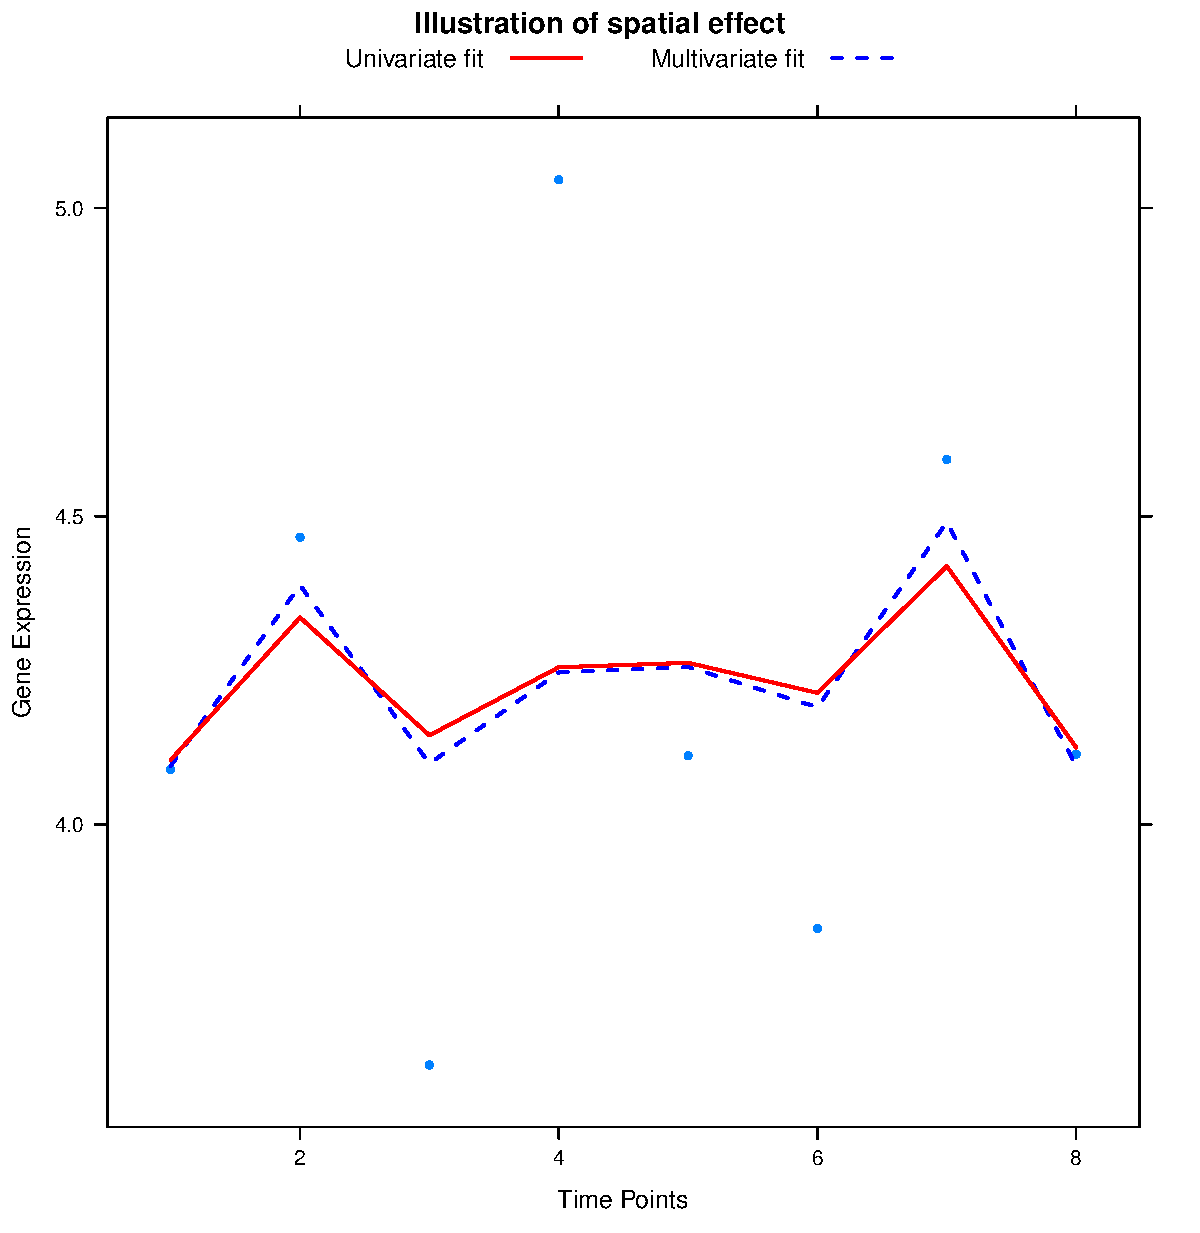
\includegraphics[scale=0.65]{Figure2.pdf}
\end{tabular}
\caption{Technical validation of microarray results by qRT-PCR for \textbf{A} mRNAs DEK, DKK3, SLC25A36 and \textbf{B} miRNAs miR-100-5p, miR-103a-3p, miR-125b-5p, miR-15b-5p and miR-221-5p. The Spearman correlation coefficient (Rho) and associated p-value (p) are indicated.}
\label{fig:figure52}
\end{figure}
\\
\\
\textbf{Validation of differential gene expression in cervical tissue samples}
\\
To investigate the in vivo relevance of our findings, expression patterns of 39 out of 106 differential miRNAs and 2661 out of 3642 differential mRNAs could be obtained from in-house available microarray data of normal HPV-positive cervical epithelium, high-grade precancerous lesions (CIN2/3) and squamous cell carcinomas (SCC, \cite{Wilting2013} and unpublished data). A concordant significant pattern of up- or downregulation was observed from normal to CIN to SCC by Spearman correlation for 24$\%$ of investigated mRNAs and 49$\%$ of investigated miRNAs. No significant up- or downward trend was observed for 62$\%$ of mRNAs and 33$\%$ of miRNAs, whereas 15$\%$ of mRNAs and 18$\%$ of miRNAs showed an opposite expression pattern in tissues compared to the cell line model.
Figure \ref{fig:figure55} shows ID1 and PITX2 as examples for mRNAs with increased or decreased expression, respectively. Deregulated miRNAs are represented by miR-4284-5p and miR-218-5p. For PITX2 and miR-4284-5p a copy number effect can be observed (fitted model with copy number effect).
\begin{figure}[h!]
\centering
\begin{tabular}{cc} 
\includegraphics[scale=0.6]{Figure5.pdf}
\end{tabular}
\caption{Deregulated mRNAs and miRNAs. Representative mRNAs (ID1, PITX2) and miRNAs (miR-4284, miR-218-5p) for increased and decreased expression are shown. Fitted models represent curves obtained using methodology from \cite{Miok2014}. If red and blue lines are similar (ID1, miR-218-5p), there is no effect of copy number on gene expression.
}
\label{fig:figure55}
\end{figure}
\\
\\
\textbf{Pinpointing key regulators in enriched pathways}
\\
Based on the unsupervised hierarchical cluster results we hypothesized that a substantial proportion of the above described DNA copy number induced gene expression changes are involved in the acquisition of anchorage independence. Indeed, 3 of the most significantly overrepresented pathways among all DNA copy number associated genes (Table \ref{table:table4}), focal adhesion, TGF-$\beta$ and mTOR signalling, are implicated in processes underlying anchorage independence (i.e. anoikis resistance and induction of EMT) \cite{Paoli2013, Frisch2013}. To further investigate this we translated our longitudinal data into pathway-based networks for focal adhesion (KEGG hsa04510), TGF-$\beta$ signalling (KEGG hsa04350) and mTOR signalling (KEGG hsa04150) (Table \ref{table:table4} and Materials $\&$ Methods section). Data-driven longitudinal networks were built for all genes in the respective pathways taking copy number into account and key regulators were identified for all 3 pathways (Table \ref{table:table2}, Figure \ref{fig:figure53}).%, Suppl. Table 5).
\begin{figure}[h!]
\centering
\begin{tabular}{cc} 
\includegraphics[scale=0.65]{Figure3.pdf}
\end{tabular}
\caption{Networks of the \textbf{A} focal adhesion, \textbf{B} mTOR signalling, and \textbf{C} TGF-$\beta$ signalling pathways. Nodes represent the genes, while the lines interaction among the genes at different time point. Dashed lines represent negative effect, while solid lines positive effect. The $X_t$ indicate copy number effect measured at time point $t$, while $Y_t$ and $Y_{t+1}$ gene expression at current and next time point.}
\label{fig:figure53}
\end{figure}
\\
\\
\textbf{Identification of potential miRNA-mRNA target interactions}
\\
Using our developed {\tt tigaR} framework we were also able to further investigate the relation between miRNA and mRNA expression in a longitudinal fashion. For this analysis we focused on the 86 miRNAs for which altered expression was either validated or not measured in the tissue specimens (excluding 20 miRNAs with non-significant changes or opposite changes in tissues). For 44 miRNAs no significant associations were found with any of the mRNA genes, whereas an additional 3 miRNAs were only displaying positive associations. When restricting the analysis to miRNA-mRNA pairs showing significant changes in expression over time in the opposite direction, 634 interactions between 27 miRNAs and 372 mRNAs remained. To verify these 634 potential interactions, we used 3 up-to-date publicly available target prediction databases ((RNA22 v2.0 \cite{Miranda2006}, miRDB v5 \cite{Wong2015}, and TargetScan v7 \cite{Agarwal2015}). Four interactions were predicted by all 3 databases (Table \ref{table:table3}), 61 interactions were predicted twice, and 225 interactions were predicted once, whereas the remainder (344 interactions) were not predicted by any of the databases. %(Suppl. Table 6). 

\begin{table}[htbp]
  \centering
  \caption{Top four predicted interactions of down-regulated miRNA and up-regulated mRNA, using data bases TargetScan\_v7, miRDB\_v5, RNA22 v2.0. Last column represent counts, number of data bases where interactions are predicted.}
    \begin{tabular}{lcccccc}
   \hline
    \hline
    \textbf{Pred. interactions} & \textbf{miR} & \textbf{mRNA} & \textbf{TargetScan} & \textbf{miRDB} & \textbf{RNA22} & \textbf{Ct} \\
    \hline
    miR-221-3p\_BRWD3 & down  & up    & target & target & target & 3 \\
    miR-221-3p\_FOS & down  & up    & target & target & target & 3 \\
    miR-30a-3p\_PECR & down  & up    & target & target & target & 3 \\
    miR-138-5p\_PLXNB2 & down  & up    & target & target & target & 3 \\
    \hline
    \hline
    \end{tabular}%
  \label{table:table3}%
\end{table}%

We selected one of the four 3 times predicted interactions, miR-221-3p\_BRWD3, for further functional validation, since miR-221-3p is known for its dual role in cancer as oncomiR and tumor suppressor miRNA \cite{Garofalo2012} and upregulation of the chromatin modifier BRWD3 was observed in cervical precancerous lesions and SCCs as well as in our model system \cite{Boon2015}. Ectopic overexpression of the miR-221-3p in late FK18B cells ($\sim$ passage 190) resulted in a 40$\%$ reduction of BRWD3 expression (Figure \ref{fig:figure54}A). As is shown in Figure \ref{fig:figure54}B, co-transfection of pmiRGLO\_BRWD3\_3UTR and ectopic miR-221-3p in Hek293 cells decreased luciferase activity compared to either co-transfection of pmiRGLO\_BRWD3\_3UTR with a non-targeting control sequence or the empty pmiRGLO vector with ectopic miR-221-3p. Directed mutagenesis of the predicted miR-221-3p seed sequence (pmiRGLO\_BRWD3\_3UTR-mut) abolished the reduction in luciferase activity observed with the wild type vector.

\begin{figure}[h!]
\centering
\begin{tabular}{cc} 
\includegraphics[scale=0.6]{Figure4.pdf}
\end{tabular}
\caption{\textbf{A} Effect of miR-221-3p on BRWD3 mRNA levels as determined by qRT-PCR in late FK18B cells (ca. passage 190). Mimic control 2 (cntr$\#$2) was used as negative transfection control, data was normalized to snRNP U1A. \textbf{B} Dual-luciferase reporter assay in Hek293 cells transiently transfected with a ne negative control (cntr$\#$1) or miR-221-3p in combination with either an empty pmiRGLO vector, a pmiRGLO-BRWD3-3UTR construct or a pmiRGLO-BRWD3-3UTR construct with mutated binding site of miR-221-3p (pmiRGLO-BRWD3-3UTR\_mut).}
\label{fig:figure54}
\end{figure}

\section{Discussion}

We here present one of the most extensive studies characterizing HPV-induced transformation over time. Chromosomal, mRNA and miRNA expression profiles were obtained from 4 individual HPV-transformed keratinocyte cell lines at 8 different time points. The obtained unique longitudinal multi-level dataset allowed for the identification of key regulators of disturbed pathways and the detection of miRNA-mRNA interactions in HPV-induced transformation. Importantly, HPV-transformed keratinocytes have previously been shown to provide useful model systems to study chromosomal instability in cancer in general \cite{Korzeniewski2011, Duensing2002}, indicating that insights on the sequential order of crucial molecular events gained in HPV-induced transformation might not only provide a better understanding of cervical cancer development, but could be applicable to other cancers too. 

Contrary to previous reports, we found that approximately one third of expression changes were directly associated to copy number, irrespective of RNA class (mRNA or miRNA) investigated. Medina-Martinez et al. found that 12.0$\%$ (241 out of 2010) differentially expressed mRNAs were related to copy number in HPV16-positive cervical tissue samples and in our cervical tissue data only a small minority of differentially expressed miRNAs was linked to copy number (5 out of 106 = 4.7$\%$) \cite{Wilting2013, Kanehisa2000, Miok2017, Livak2001, Wilting2016, Paoli2013, Frisch2013, Garofalo2012, Boon2015, Korzeniewski2011, Duensing2002, Medina2014}. Moreover, the expression of only 2 miRNAs was influenced by copy number in hematopoietic cell lines, suggesting that there is little correlation between copy number and miRNA expression \cite{Veigaard2014}. On the other hand, \cite{Zhang2006} identified 41 miRNA genes with copy number changes that were shared between melanoma, ovarian and breast cancer and many more miRNA genes with copy number changes that were unique to each of the epithelial tumor types \cite{Zhang2006}. In accordance with our data, copy number losses were reported to account for the down-regulation of approximately 15$\%$ of miRNAs in advanced ovarian tumors \cite{Zhang2008}. Discrepancies between studies can be explained by the multitude of different experimental approaches and statistical methods used to study the association between copy number and miRNA expression. While most studies analyzed cross-sectional clinical material or a number of cell lines, we here had the unique opportunity to follow copy number and gene expression changes within the specific cellular background of our 4 transforming cell lines over time. In addition, we cannot exclude that the large fraction of copy number induced expression changes found in our study is specific to cervical carcinogenesis and that copy number changes might have less impact on mRNA and miRNA expression in a different context.

Besides studying the effect of copy number aberrations on gene expression, our previously developed {\tt tigaR} framework also proved suitable for the identification of miRNA-mRNA interactions\cite{Miok2014}. We identified a total of 634 potential miRNA-mRNA interactions and validated the miR-221-3p\_BRWD3 interaction on RNA level and by dual-luciferase assay. 

As described before unsupervised hierarchical clustering of our miRNA expression data separated well between anchorage-dependent and independent passages of our transformed keratinocyte cell lines \cite{Wilting2016}, but the role of chromosomal alterations in the acquisition of anchorage independence was even more eminent. Anchorage-independent cell growth is a hallmark of transformation in vitro \cite{Freedman1974, Mori2009}. While loss of appropriate cell-cell and cell-matrix interactions leads to aberrant integrin signalling and eventually detachment-induced cell death (anoikis) in healthy epithelial cells, cancerous epithelial cells overcome anoikis by epithelial-to-mesenchymal transition (EMT), activation of survival and proliferation pathways or temporary dormancy \cite{Guadamillas2011}. In HPV-transformed cells, silencing of a number of tumour suppressor genes (including miRNAs) was shown to contribute to anchorage-independence \cite{Wilting2016, Khalifa2011, Mack2013, Overmeer2009, Razani2000, Steenbergen2004}). Our clustering results suggest that anchorage-independent cell growth represents highly relevant functional read-out when studying the effect of molecular changes on transformation in vitro.

Pathway enrichment analysis on copy number affected mRNAs identified focal adhesion, mTOR signalling and TGF-$\beta$ signalling as the top 3 altered pathways in HPV-induced carcinogenesis. Strikingly, all 3 pathways are implicated in anoikis resistance and induction of EMT \cite{Paoli2013, Frisch2013, Garofalo2012}, again suggesting that the acquisition of anchorage independence in HPV-induced transformation is largely driven by chromosomal changes. It is therefore not surprising that extracellular matrix proteins such as LAMA4 (laminin subunit alpha 4), COL5A3 (collagen type V alpha 3) and motor protein MYLPF (myosin light chain, phosphorylatable, fast skeletal muscle) were among the key regulators of focal adhesion signalling. Consistent with the here observed downregulation of LAMA4, it has previously been shown that ectopic overexpression of LAMA4 resulted in increased cellular adhesion in anchorage-independent cervical cancer cell line HeLa54. Similarly, the here identified key regulators of the mTOR pathway IGF1 (insulin like growth factor 1) and HIF1A (hypoxia inducible factor 1 alpha subunit) were previously described to be involved anoikis resistance in hepatocellular carcinoma cells \cite{Tang2015, Sun2014}. HIF1A also upregulates EMT inducers such as SNAI1, TWIST and SIP1 \cite{Luo2011, Yang2008, Evans2007}). TGF-$\beta$1 has been reported to exert a tumor inhibiting function in early stages of cervical carcinogenesis, while it plays an oncogenic role at a later stage by promotion of EMT and metastasis, induction of angiogenesis and escape from immune surveillance \cite{Zhu2016}. In line with this, expression of TGF-$\beta$1 was found to be downregulated in cervical precancerous lesion compared to normal epithelium although it is increased in cervical cancers \cite{Wu2002, Hou2012, Fan2014}. This TGF-$\beta$ paradox is not unique to cervical carcinogenesis but has been recognized in many other cancers as well \cite{Massague2008, Neuzillet2015, Shen2017}. A number of TGF-$\beta$ and TGF-$\beta$ receptor inhibitors is currently being tested for the treatment of a variety of cancers in phase I-IV clinical trials \cite{Colak2017}. In cervical cancer, a negative correlation between pre-radiation TGF-$\beta$1 levels and radiosensitivity suggests that tumor response can be increased by inhibition of TGF-$\beta$1 prior to radiation \cite{Zhu2016}.

We here present a unique longitudinal multi-level dataset on HPV-induced transformation. Using state-of-the-art analysis tools, we identified key pathway regulators and potential miRNA-mRNA interactions relevant to the carcinogenic process. Our results highlight the importance of chromosomal alterations for the acquisition of anchorage independence during transformation. Additional functional studies on the identified key pathway regulators and differentially expressed m(i)RNAs will likely result in many more potential therapeutic targets and disease markers in the future.
\begin{table}[htbp]
  \centering
  \caption{Network enrichment analysis of copy number related genes in 118 KEGG pathways.}
    \begin{tabular}{lccc}
    \hline\hline
    & \multicolumn{1}{l}{\textbf{Nr. of }} & \multicolumn{1}{l}{\textbf{\% of CN      }} & \multicolumn{1}{l}{\textbf{Adj.}} \\
    \multicolumn{1}{c}{\textbf{keggName}} & \multicolumn{1}{l}{\textbf{genes in}} & \multicolumn{1}{l}{\textbf{related}} & \multicolumn{1}{l}{\textbf{P-value}} \\
    & \multicolumn{1}{p{3.89em}}{\textbf{pathway}} & \multicolumn{1}{p{4.39em}}{\textbf{genes}} & \multicolumn{1}{p{4.165em}}{\textbf{ (Chi2)}} \\
    \hline
    \rowcolor[rgb]{ 1,  1,  0}  Focal adhesion & 200   & 7.50  & 0.0001 \\
    \rowcolor[rgb]{ 1,  1,  0}  TGF-beta signaling pathway & 85    & 5.88  & 0.0152 \\
    \rowcolor[rgb]{ 1,  1,  0}  mTOR signaling pathway & 52    & 5.77  & 0.0268 \\
    Nucleotide excision repair & 45    & 4.44  & 0.0000 \\
    Mismatch repair & 23    & 4.35  & 0.0003 \\
    p53 signaling pathway & 69    & 4.35  & 0.0008 \\
    Wnt signaling pathway & 151   & 3.31  & 0.0018 \\
    Biosynthesis of unsaturated fatty acids & 21    & 4.76  & 0.0019 \\
    Neurotrophin signaling pathway & 127   & 3.15  & 0.0033 \\
    B cell receptor signaling pathway & 75    & 8.00  & 0.0036 \\
    Cell cycle & 128   & 7.81  & 0.0038 \\
    Glycosaminoglycan biosynthesis & 26    & 7.69  & 0.0242 \\
    Glycosylphosphatidylinositol(GPI) & 25    & 8.00  & 0.0242 \\
    N-Glycan biosynthesis & 49    & 6.12  & 0.0245 \\
    Purine metabolism & 162   & 4.32  & 0.0268 \\
    Glutathione metabolism & 50    & 8.00  & 0.0268 \\
    mRNA surveillance pathway & 83    & 0.00  & 0.0271 \\
    Synthesis and degradation of ketone bodies & 9     & 11.11 & 0.0311 \\
    Aminoacyl-tRNA biosynthesis & 63    & 3.17  & 0.0400 \\
    Thiamine metabolism & 4     & 0.00  & 0.0487 \\
    Lipoic acid metabolism & 3     & 0.00  & 0.0487 \\
    \midrule
    Apoptosis & 89    & 4.49  & 0.0542 \\
    Valine  leucine and isoleucine degradation & 44    & 2.27  & 0.0563 \\
    Alanine  aspartate and glutamate metabolism & 32    & 15.63 & 0.0606 \\
    T cell receptor signaling pathway & 108   & 6.48  & 0.0731 \\
     Pyrimidine metabolism & 99    & 2.02  & 0.0774 \\
     Porphyrin and chlorophyll metabolism & 43    & 4.65  & 0.0913 \\
    Phosphatidylinositol signaling system & 78    & 2.56  & 0.0913 \\
     Sphingolipid metabolism & 40    & 2.50  & 0.0913 \\
     Ribosome biogenesis in eukaryotes & 81    & 1.23  & 0.1173 \\
     Glycosphingolipid biosynthesis & 26    & 7.69  & 0.1373 \\
     ECM-receptor interaction & 85    & 7.06  & 0.1373 \\
    Fatty acid metabolism & 43    & 2.33  & 0.1451 \\
     ErbB signaling pathway & 87    & 3.45  & 0.1504 \\
     Inositol phosphate metabolism & 57    & 1.75  & 0.1942 \\
    \hline\hline
\end{tabular}%
  \label{table:table4}%
\end{table}%

